\section{Motivation}

\begin{itemize}
\item ``Throw hardware at the problem''.
\item No linear scalability demonstrated with previous approaches. Main cause: imbalanced tree shape, unknown a priori.
\item Foundation for a software testing service.
\end{itemize}

Testing a program consists of exercising many different paths through it and checking whether they ``do the right thing.''  In other words, testing is a way to produce partial evidence of correctness, and thus increase confidence in the tested software.  Yet, due to the typically poor coverage one can get today, testing often turns into a mere hunt for bugs.

In practice, most software test harnesses consist of manually written tests that are run periodically; regression test suites provide an automated way of checking whether new bugs have entered the code~\cite{codeComplete}.  Such suites tend to be tedious to write and maintain but, once in place, they can be reused and extended.  In practice, the state of the art consists mostly of fuzzing, i.e., trying various inputs in the hope of finding bugs and improving test coverage.

In research, the state of the art consists of model checkers and automated test generators based on symbolic execution~\cite{dart,klee}.  Instead of running a program with regular concrete inputs (e.g., $x\!=\!5$), symbolic execution consists of running a program with ``symbolic'' inputs that can take on all values allowed by the type (e.g., $x\!=\!\lambda$, where $\lambda \in \mathbb{N}$).  Whenever a conditional branch is encountered that involves a predicate $\pi$ that depends (directly or indirectly) on $x$, state and execution are forked into two alternatives: one following the then-branch ($\pi$) and another following the else-branch ($\neg \pi$). The two executions can now be pursued independently.  When a bug is found, test generators can compute concrete values for program inputs that take the program to the bug location.  This approach is efficient because it analyzes code for entire classes of inputs at a time, thus avoiding the redundancy inherent in fuzzing.

The {\em first challenge} for such tools is path explosion, as mentioned earlier.  One way to cope is to memoize the symbolic execution of sub-paths into test summaries that can be subsequently reused when the same sub-path is encountered again, as done in compositional test generation~\cite{godefroid:compdyntest}.  Alternatively, it is possible to use various heuristics to prioritize the most interesting paths first, as done in \klee~\cite{klee}.  Another approach is to execute symbolically only paths that are of interest to the test, as done in selective symbolic execution~\cite{s2e}.

We pursue a complementary approach---{\em parallel symbolic execution}---in which we symbolically execute a program in parallel on a cluster, thus harnessing the machines into a ``distributed computer'' whose aggregate CPU and memory surpass that of an individual machine.  An alternative to a cluster-based approach would be to run a classic single-node symbolic execution engine on a Blue Gene-like supercomputer with vast shared memory and CPUs communicating over MPI.  Supercomputers, however, are expensive, so we favor instead clusters of cheap commodity hardware.  

One way to parallelize symbolic execution is by statically dividing up the task among nodes and having them run independently.   However, when running on large programs, this approach leads to high workload imbalance among nodes, making the entire cluster proceed at the pace of the slowest node~\cite{parallelSymbex}.  If this node gets stuck, for instance, while symbolically executing a loop, the testing process may never terminate.  Parallelizing symbolic execution on shared-nothing clusters in a way that scales well is difficult.

The {\em second challenge} is mediating between a program and its environment, i.e., symbolically executing a program that calls into libraries and the OS, or communicates with other systems, neither of which execute symbolically.  One possible approach is to simply allow the call to go through into the ``concrete'' environment (e.g., to write a file)~\cite{dart,exe}; unfortunately, this causes the environment to be altered for \emph{all} forked executions being explored in parallel, thus introducing inconsistency.  Another approach is to replace the real environment with a symbolic model, i.e., a piece of code linked with the target program that provides the illusion of interacting with a symbolically executing environment.  For instance, \klee uses a symbolic model of the file system~\cite{klee}. Of course, real-world programs typically interact in richer ways than just file I/O: they fork processes, synchronize threads, etc.  

We originally viewed the building of a complete environment model as an engineering task, but our ``mere engineering'' attempt failed: for any functionality that, in a normal execution, requires hardware support (such as enforcing isolation between address spaces), the core symbolic execution engine had to be modified.  The research challenge therefore is to find the minimal set of engine primitives required to support a rich model of a program's environment. 

The {\em third challenge} is using an automated test generator in the context of a development organization's quality assurance processes.  To take full advantage of the automated exploration of paths, a testing tool must provide ways to control all aspects of the environment.  For example, there needs to be a clean API for injecting failures at the boundary between programs and their environment, there must be a way to control thread schedules, and so on.  There should be a way to programmatically orchestrate all environment-related events, but doing so should not require deep expertise in the technology behind the testing tools themselves.

The work presented here aims to address these three challenges.  Cluster-based parallel symbolic execution (Section~\ref{ch:parsymbex}) provides the illusion of running a classic symbolic execution engine on top of a large, powerful computer.  Without changing the exponential nature of the problem, parallel symbolic execution harnesses cluster resources to make it feasible to run automated testing on larger systems than what was possible until now. Our work complements and benefits all tools and approaches based on symbolic execution.  We describe a way to accurately model the environment (Section~\ref{ch:cloud9}) with sufficient completeness to test complex, real software, like the Apache web server and the Python interpreter.  We present the APIs and primitives that we found necessary in developing a true testing platform (Section~\ref{sec:platform}).  We show how using these APIs enables, for instance, finding errors in bug patches by reproducing environment conditions which otherwise would have been hard or impossible to set up with regular test cases.

In this section we present the design of the \cnine engine, focusing on the algorithmic aspects: after a conceptual overview (Section~\ref{sec:concept}), we describe how \cnine operates at the worker level (Section~\ref{sec:workerView}) and then at the cluster level (Section~\ref{sec:loadBalancing}).

%%%%%%%%%%%%%%%%%%%%%%%%%%%%%%%%%%%%%%%%%%%%%%%%%%%%%%%%%%%%%%%%%%%%%%%%%%%%%%%%

\section{Overview}
\label{sec:concept}

\begin{itemize}
\item Introduce workers + load balancer.
\item Goal: disjoint and complete tree exploration.
\item Each worker explores tree independently, with minimal synchronization overhead.
\end{itemize}

%--------------------------------------------------
\paragraph{Classic Symbolic Execution}

\cnine employs symbolic execution, an automated testing technique that has recently shown a lot of
promise~\cite{dart,klee}. 

A symbolic execution engine (SEE) executes a program with unconstrained symbolic inputs.  When a branch involves symbolic values, execution forks into two parallel executions (see Section~\ref{sec:overview}), each with a corresponding clone of the program state.  Symbolic values in the clones are {\em constrained} to make the branch condition evaluate to false (e.g., $\lambda\!\ge${\small MAX}) respectively true (e.g., $\lambda\!<${\small MAX}). Execution recursively splits into sub-executions at each subsequent branch, turning an otherwise linear execution into an {\em execution tree} (Fig.~\ref{fig:exectree}). 

\begin{figure}[h!]
  \centering
  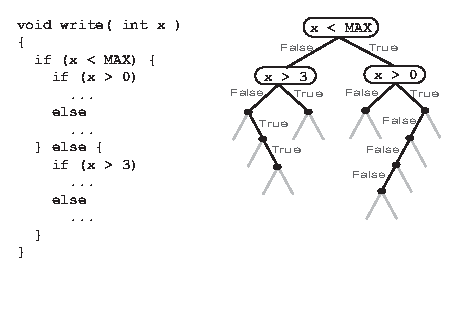
\epsfig{file=figures/parsymbex/execTree.eps, width=2.7in}
  \vspace{-10mm}
  \caption{Symbolic execution produces an execution tree.}
  \label{fig:exectree}
  \vspace{-2mm}
\end{figure}

In this way, all execution paths in the program are explored.  To ensure that only feasible paths are explored, the SEE uses a constraint solver to check the satisfiability of each branch's predicate, and it only follows satisfiable branches.  If a bug is encountered (e.g., a crash or a hang) along one of the paths, the solution to the constraints accumulated along that path yields the inputs that take the tested program to the bug---these inputs constitute a {\em test case}.

%--------------------------------------------------
\paragraph{Parallel Symbolic Execution}

Since the size of the execution tree is exponential in the number of branches, and the complexity of constraints increases as the tree deepens, state-of-the-art SEEs can quickly bottleneck on CPU and memory even for programs with just a couple \kloc.  We therefore build a parallel SEE that runs on a commodity cluster and enables ``throwing hardware at the problem.''

The key design goal is to enable individual cluster nodes to explore the execution tree independently of each other.  One way of doing this is to statically split the execution tree and farm off subtrees to worker nodes.  Alas, the contents and shape of the execution tree are not known until the tree is actually explored, and finding a balanced partition (i.e., one that will keep all workers busy) of an unexpanded execution tree is undecidable.  Besides subtree size, the amount of  memory and CPU required to explore a subtree is also undecidable, yet must be taken into account when partitioning the tree. Since the methods used so far in parallel model checkers~\cite{swarm,spin:multicore-modelchecking} rely on static partitioning of a finite state space, they cannot be directly applied to the present problem. Instead, \cnine partitions the execution tree {\em dynamically}, as the tree is being explored. 

%--------------------------------------------------
\paragraph{Dynamic Distributed Exploration}

\cnine consists of wor\-ker nodes and a load balancer (LB).  Workers run independent SEEs, based on \klee~\cite{klee}.  They explore portions of the execution tree and send statistics on their progress to the LB, which in turn instructs, whenever necessary, pairs of workers to balance each other's work load.  Encoding and transfer of work is handled directly between workers, thus taking the load balancer off the critical path.

The goal is to dynamically partition the execution tree such that the parts are {\em disjoint} (to avoid redundant work) and together they {\em cover} the global execution tree (for exploration to be complete).  We aim to minimize the number of work transfers and associated communication overhead.  A fortuitous side effect of dynamic partitioning is the transparent handling of fluctuations in resource quality, availability, and cost, which are inherent to large clusters in cloud settings.

\cnine operates roughly as follows: The first component to come up is the load balancer.  When the first worker node $W_1$ joins the \cnine cluster, it connects to the LB and receives a ``seed'' job to explore the entire execution tree.  When the second worker $W_2$ joins and contacts the LB, it is instructed to balance $W_1$'s load, which causes $W_1$ to break off some of its unexplored subtrees and send them to $W_2$ in the form of {\em jobs}.  As new workers join, the LB has them balance the load of existing workers.  The workers regularly send to the LB status updates on their load in terms of exploration jobs, along with current progress in terms of code coverage, encoded as a bit vector.  Based on workers' load, the LB can issue job transfer requests to pairs of workers in the form $\langle$~source worker, destination worker, \# of jobs~$\rangle$.  The source node decides which particular jobs to transfer.

%%%%%%%%%%%%%%%%%%%%%%%%%%%%%%%%%%%%%%%%%%%%%%%%%%%%%%%%%%%%%%%%%%%%%%%%%%%%%%%%

\section{Worker-level Operation}
\label{sec:workerView}

\begin{itemize}
\item Introduce dead, fence, and candidate nodes.
\end{itemize}

A worker's visibility is limited to the subtree it is exploring locally.  As $W_i$ explores and reveals the content of its local subtree, it has no knowledge of what $W_j$'s ($i\ne j$) subtree looks like.  No element in the system---not even the load balancer---maintains a global execution tree.  Disjointness and completeness 
of the exploration (see Fig.~\ref{fig:architecture}) are ensured by the load balancing algorithm.

\begin{figure}[h!]
  \centering
  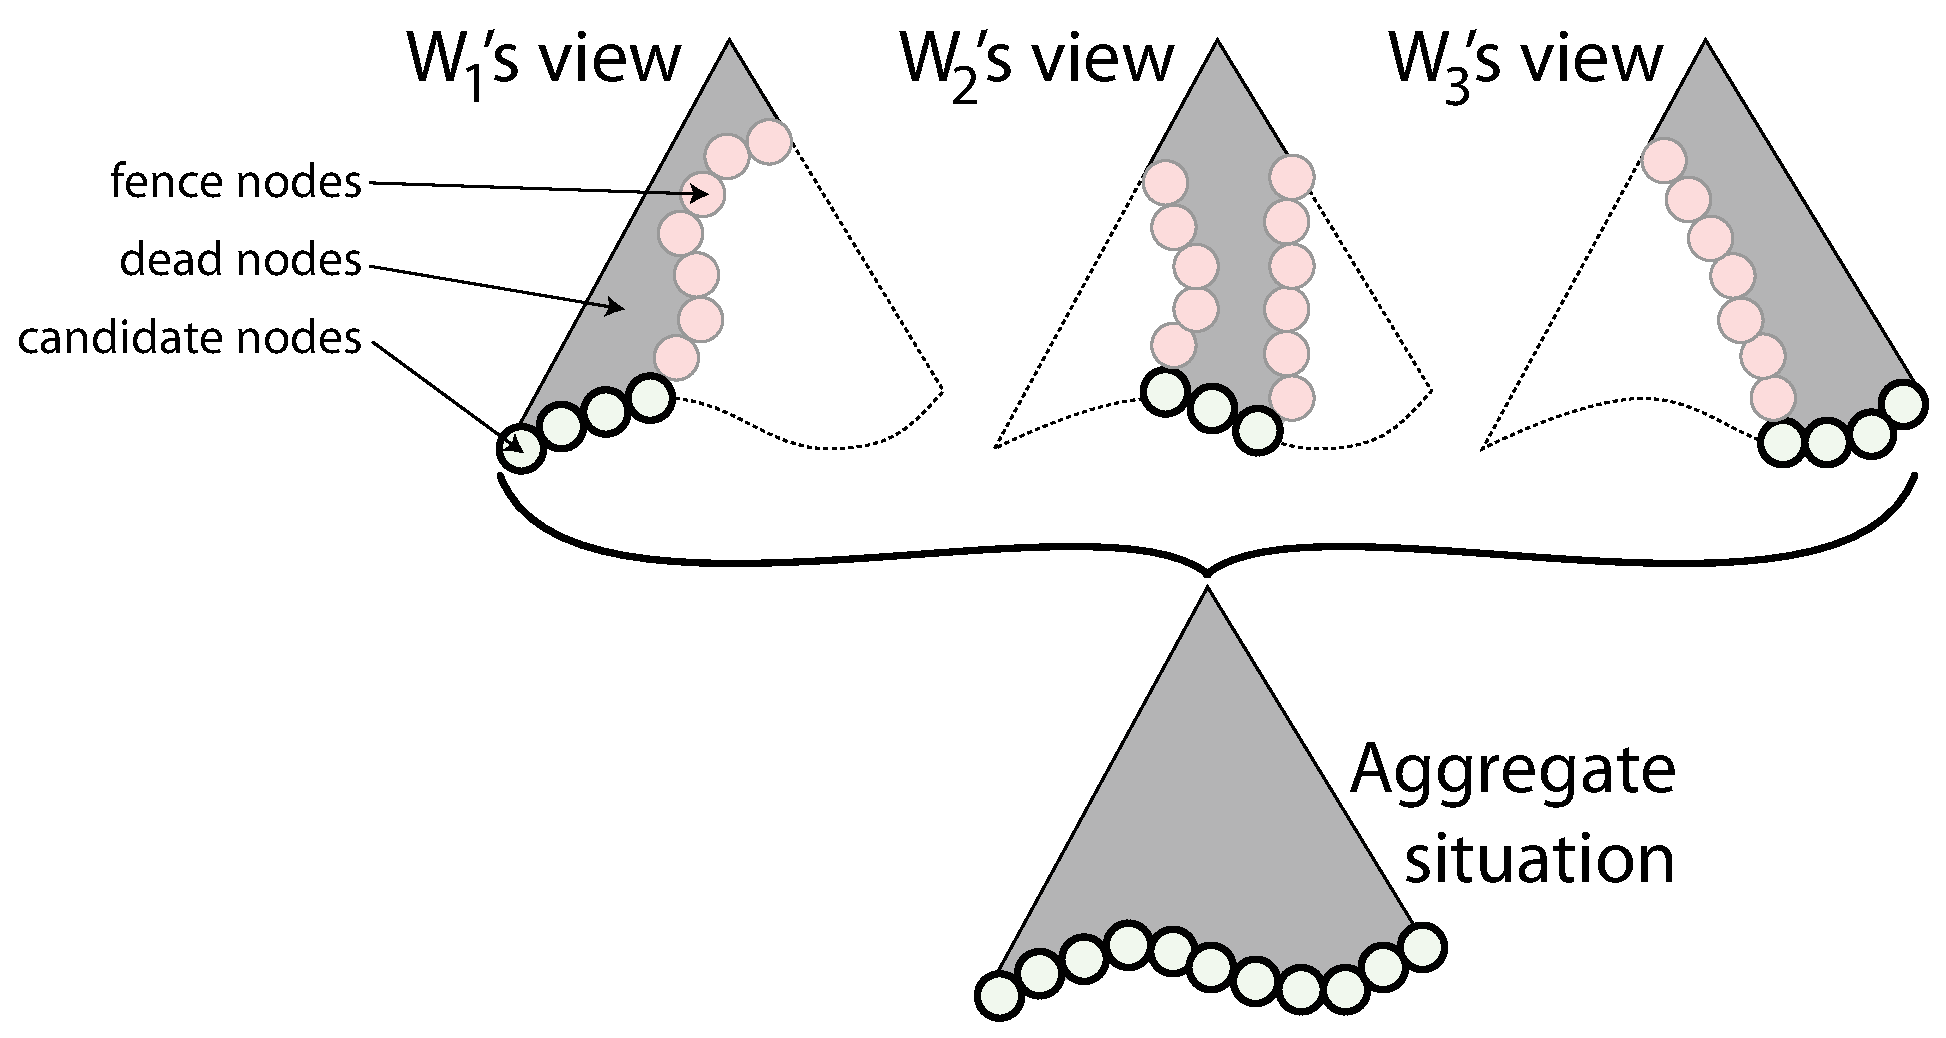
\epsfig{file=figures/parsymbex/architecture-parsymbex, height=1.7in}
  \caption{Dynamic partitioning of exploration in \cnine.}
 \label{fig:architecture}
\end{figure}

\newcommand{\dead}{dead\xspace}
\newcommand{\fence}{fence\xspace}
\newcommand{\candidate}{candidate\xspace}
\newcommand{\virtual}{virtual\xspace}
\newcommand{\materialized}{materialized\xspace}

As will be explained later, each worker has the root of the global execution tree.  The tree portion explored thus far on a worker consists of three kinds of nodes: (1) internal nodes that have already been explored and are thus no longer of interest---we call them {\em \dead} nodes; (2) {\em \fence} nodes that demarcate the portion being explored, separating the domains of different workers; and (3) {\em \candidate} nodes, which are nodes ready to be explored.  A worker exclusively explores \candidate nodes; it never expands \fence or \dead nodes.

Candidate nodes are leaves of the local tree, and they form the \emph{exploration frontier}.  The work transfer algorithm ensures that frontiers are disjoint between workers, thus ensuring that no worker duplicates the exploration done by another worker.  At the same time, the union of all frontiers in the system corresponds to the frontier of the global execution tree. The goal of a worker  $W_i$ at every step is to choose the next \candidate node to explore and, when a bug is encountered, to compute the inputs, thread schedule, and system call returns that would take the program to that bug.

 The implementation of this conceptual model lends itself to many optimizations, some of which we cover in Section~\ref{sec:implementation}.  Broadly speaking, judicious use of copy-on-write and a novel state-encoding technique ensure that actual program state is only maintained for \candidate and \fence nodes.

%--------------------------------------------------
\paragraph{Worker-to-Worker Job Transfer}
\label{sec:workTransfer}

\newcommand{\wsrc}{\ensuremath{W_s}\xspace}
\newcommand{\wdst}{\ensuremath{W_d}\xspace}

When the global exploration frontier becomes poorly balanced across workers, the load balancer chooses a loaded worker \wsrc and a less loaded worker \wdst  and instructs them to balance load by sending $n$ jobs from \wsrc to \wdst.  In the extreme, \wdst is a new worker or one that is done exploring its subtree and has zero jobs left.  

\wsrc chooses $n$ of its \candidate nodes and packages them up for transfer to \wdst.  Since a \candidate node sent to another worker is now on the boundary between the work done by \wsrc and the work done by \wdst, it becomes a \fence node at the sender.  This conversion prevents redundant work.

A job can be sent in at least two ways: (1) serialize the content of the chosen node and send it to \wdst, or (2) send to \wdst the path from the tree root to the node, and rely on \wdst to ``replay'' that path and obtain the contents of the node.  Choosing one vs. the other is a trade-off between time to encode/decode and network bandwidth: option (1) requires little work to decode, but consumes bandwidth (the state of a real program is typically at least several megabytes), while encoding a job as a path requires replay on \wdst.  We assume that large commodity clusters have abundant CPU but meager bisection bandwidth,
so in \cnine we chose to encode jobs as the path from the root to the \candidate node.  As an optimization, we exploit common path prefixes: jobs are not encoded separately, but rather the corresponding paths are aggregated into a job tree and sent as such.

\begin{wrapfigure}{r}{1in}
\vspace{-5mm}
%
%\includegraphics[height=50mm]{new-diagrams/worker-tree-thumb}
\hspace{-10mm}\includegraphics[height=50mm]{figures/parsymbex/worker-tree-thumb}
%\caption{Example of a local worker tree.}
\vspace{-8mm}
\end{wrapfigure}

When the job tree arrives at \wdst, it is imported into \wdst's own subtree, and the leaves of the job tree become part of \wdst's frontier (at the time of arrival, these nodes may lie ``ahead'' of \wdst's frontier).  \wdst keeps the nodes in the incoming jobs as {\em \virtual} nodes, as opposed to {\em \materialized} nodes that reside in the local subtree, and replays paths only lazily.  A \materialized node is one that contains the corresponding program state, whereas a \virtual node is an ``empty shell'' without corresponding program state.  In the common case, the frontier of a worker's local subtree contains a mix of \materialized and \virtual nodes, as shown in the diagram above.

As mentioned earlier, a worker must choose at each step which \candidate node to explore next---this choice is guided by a {\em strategy}.  Since the set of \candidate nodes now contains both \materialized and \virtual nodes, it is possible for the strategy to choose a \virtual node as the next one to explore.  When this happens, the corresponding path in the job tree is replayed (i.e., the symbolic execution engine executes that path); at the end of this replay, all nodes along the path are \dead, except the leaf node, which has converted from \virtual to \materialized and is now ready to be explored.  Note that, while exploring the chosen job path, each branch produces child program states; any such state that is not part of the path is marked as a \fence node, because it represents a node that is being explored elsewhere, so \wdst should not pursue it.

\paragraph{Summary}

\newcommand{\status}{\ensuremath{\mathrm{status}}\xspace}
\newcommand{\alive}{\ensuremath{\mathrm{life}}\xspace}

A node $N$ in $W_i$'s subtree has two attributes, $N^{\status} \in$\{\materialized, \virtual\!\} and $N^{\alive} \in$\{\candidate, \fence, \dead\!\}.  A worker's frontier $F_i$ is the set of all \candidate nodes on worker $W_i$.  The worker can only explore nodes in $F_i$, i.e., \dead nodes are off-limits and so are \fence nodes, except if a \fence node needs to be explored during the replay of a job path.  The union $\cup F_i$ equals the frontier of the global execution tree, ensuring that the aggregation of worker-level explorations is complete.  The intersection $\cap F_i = \emptyset$, thus avoiding redundancy by ensuring that workers explore disjoint subtrees.  Fig.~\ref{fig:transitions} summarizes the life cycle of a node.

\begin{figure}[h!]
  \centering
  \hspace{-4mm}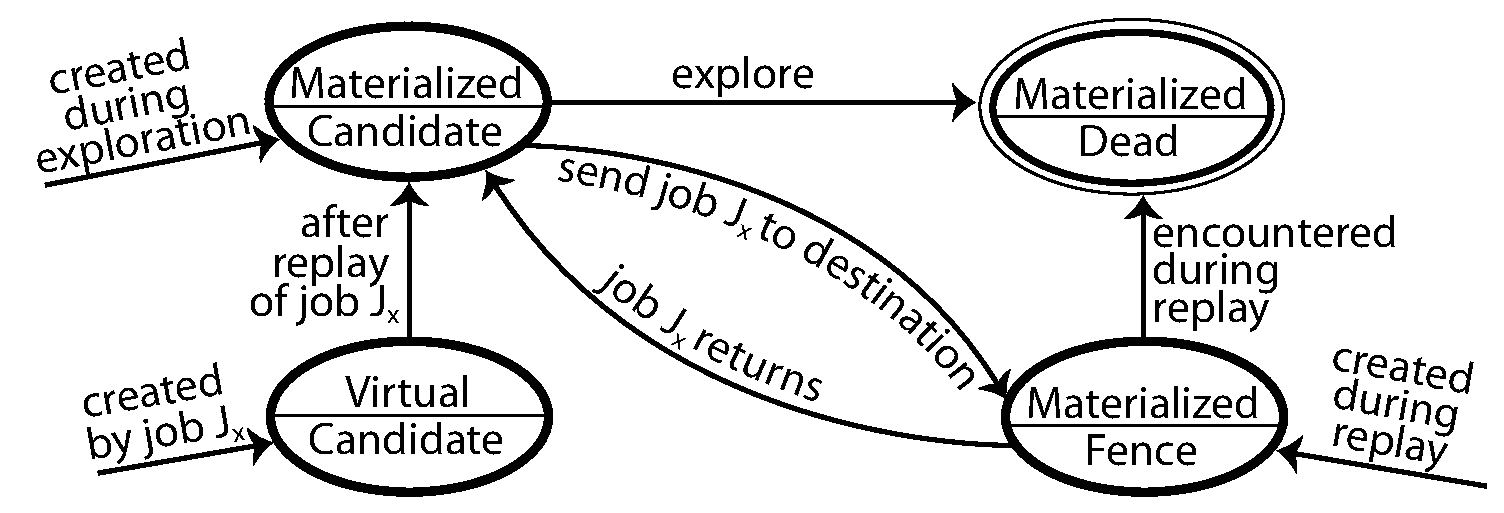
\epsfig{file=figures/parsymbex/node-transitions, width=3.4in}
  \caption{Transition diagram for nodes in a worker's subtree.}
 \label{fig:transitions}
\end{figure}

As suggested in Fig.~\ref{fig:transitions}, once a tree node is \dead, it has reached a terminal state; therefore, a dead node's state can be safely discarded from memory.  This enables workers to maintain program states only for \candidate and \fence nodes.

%%%%%%%%%%%%%%%%%%%%%%%%%%%%%%%%%%%%%%%%%%%%%%%%%%%%%%%%%%%%%%%%%%%%%%%%%%%%%%%%

\section{Cluster-level Operation}
\label{sec:loadBalancing}

\begin{itemize}
\item Describe the load balancer operation.
\end{itemize}

\paragraph{Load Balancing}

When jobs arrive at \wdst, they are placed conceptually in a queue; the \emph{length} of this queue is sent to the load balancer periodically.  The LB ensures that the worker queue lengths stay within the same order of magnitude.  The balancing algorithm takes as input the lengths $l_i$ of each worker $W_i$'s queue $Q_i$.  It computes the average $\bar{l}$ and standard deviation $\sigma$ of the $l_i$ values and then classifies each $W_i$ as underloaded ($l_i < max \{ \bar{l}-\delta \cdot \sigma, 0 \}$), overloaded ($l_i > \bar{l} + \delta \cdot \sigma$), or OK otherwise; $\delta$ is a constant factor.  The $W_i$ are then sorted according to their queue length $l_i$ and placed in a list.  LB then matches underloaded workers from the beginning of the list with overloaded workers from the end of the list.  For each pair $\langle W_i,W_j \rangle$, with $l_i < l_j$, the load balancer sends a job transfer request to the workers to  move $(l_j - l_i)/2$ \candidate nodes from $W_j$ to $W_i$.


%===========================================================================
\paragraph{Coordinating Worker-level Explorations}
\label{sec:globalStrategy}

Classic symbolic execution relies on heuristics to choose which state on the frontier to explore first, so as to efficiently reach the chosen test goal (code coverage, finding a particular type of bug, etc.). In a distributed setting, local heuristics must be coordinated across workers to achieve the global goal, while keeping communication overhead at a minimum. What we have described so far ensures that eventually all paths in the execution tree are explored, but it provides no aid in focusing on the paths desired by the global strategy.  In this sense, what we described above is a \emph{mechanism}, while the exploration strategies represent the \emph{policies}.

Global strategies are implemented in \cnine using its interface for building {\em overlays} on the execution tree structure.  We used this interface to implement distributed versions of all strategies that come with \klee~\cite{klee}; the interface is also available to \cnine users.  Due to space limitations, we do not describe the strategy interface further, but provide below an example of how a global strategy is built.

A coverage-optimized strategy drives exploration so as to maximize coverage~\cite{klee}.  In \cnine, coverage is represented as a bit vector, with one bit for every line of code; a set bit indicates that a line is covered.  Every time a worker explores a program state, it sets the corresponding bits locally. The current version of the bit vector is piggybacked on the status updates sent to the load balancer.  The LB maintains the current global coverage vector and, when it receives an updated coverage bit vector, {\small OR}s it into the current global coverage.  The result is then sent back to the worker, which in turn {\small OR}s this global bit vector into its own, in order to enable its local exploration strategy to make choices consistent with the global goal.  The coverage bit vector is an example of a \cnine overlay data structure.


%%% Local Variables: 
%%% mode: latex
%%% eval: (visual-line-mode)
%%% fill-column: 1000000
%%% TeX-master: "main"
%%% End:
